% marc_aaai.tex — AAAI-2026 main-track port of marc.tex (the corrected source of truth).
%
% Format: official AAAI-26 author kit (aaai2026.sty / aaai2026.bst, in this directory),
% wired in below via \usepackage[submission]{aaai2026}; the style sets
% \bibliographystyle{aaai2026} itself. Kit provenance: STYLE_KIT_STATUS.md.
% Content rule: port + cut of marc.tex — every number identical, all \citep keys kept.
% The technical appendix (per-family tables, transfer, K-scaling) is marc_aaai_appendix.tex,
% input after the bibliography; it is intended as supplementary material.

\documentclass[letterpaper]{article}
\usepackage[submission]{aaai2026}
\usepackage{times}
\usepackage{helvet}
\usepackage{courier}
\usepackage[hyphens]{url}
\usepackage{graphicx}
\usepackage{booktabs}
\usepackage{amsmath,amssymb}
\usepackage{natbib}
\usepackage{caption}
\frenchspacing

\title{Learn the Structure, Not the Values:\\
A Controlled Characterization of Learning in Exact Constraint Solving}
% Submission is double-blind: keep the anonymous line active until camera-ready.
% Camera-ready author block (equal contribution), swap in after acceptance:
%   \author{Quang Bui\equalcontrib, Sparsh Roy\equalcontrib,
%           Akash Gundimeda\equalcontrib, Davin Yin\equalcontrib}
%   \affiliations{SAID Laboratory}
\author{Anonymous submission}
\date{}

\begin{document}
\maketitle

\begin{abstract}
Learning pays in exact constraint solving at the discrete decision, not the continuous one.
We measure both under a single protocol. MARC encodes a system as a factor graph, proposes
assignments with a graph-neural diffusion denoiser, polishes them on an exact
computer-algebra energy, and certifies with an exact symbolic checker. The decision classical
solvers make only by enumeration is discrete --- which structural augmentation renders an
unsolvable system solvable --- and there a candidate-conditioned repair ranker matches the
exhaustive-enumeration ceiling at far fewer calls, beating random and a stronger
per-candidate probe on accuracy and cost (0.997 vs 0.236 balanced nonlinear accuracy;
$p<10^{-70}$; $0.982\pm0.006$ across seeds). The effect is not confined to menus we built:
on hardened variants of named real systems, a construction derived from the givens and
selected on held-out failures repairs every remaining failure of far-side trilateration and
of a ghost-root conic intersection, against $0.433\pm0.049$ and $0.114\pm0.011$ for restart
control matched to the full enumeration budget. On the value decision the same discipline
curtails our own earlier claim: random multi-start at identical polish and budget --- the
control such evaluations rarely include --- erases most of the learned proposal's apparent
advantage, leaving a predictable regime. It ties or loses to
random restart on trapped low-dimensional families, wins where dimension collapses random
search, and loses once variables couple. All methods share one polish and checker, so
best-of-$K$ random multi-start succeeds with probability exactly $1-(1-q(n))^K$ in the
single-start reachability $q(n)$; on the separable family one measured constant reproduces
the best-of-8 curve with no free parameters (mean absolute error 0.012), and classical
multi-start solves all eight standard test systems we encode, none of which falls in the
favorable regime. A closing geometry study
prices the trap such claims invite: single-stream failure selection makes repairs look
decisive; two-stream selection and a budget-matched screen show the residual probe advantage
is portfolio breadth, not learnable signal. We map where learning improves on classical
search, and where the win is cost over enumeration, not reach beyond it.
\end{abstract}

\section{Introduction}
\label{sec:intro}

Solving a system of algebraic constraints involves two different kinds of decision. The
continuous decision asks which values satisfy the equations; it is smooth, gradient-rich, and
has been owned by numerical analysis for sixty years. The discrete decision asks which
representation makes the problem tractable at all: which auxiliary variable, substitution, or
defining relation to introduce. Classical numerical solvers take the representation as given
and make this choice only by enumeration; for the value decision they are very hard to
beat. This paper measures both decisions under controlled conditions: learning earns its
place on the discrete one, where enumeration is the classical fallback, and helps on the
value decision only in a narrow regime we can name exactly.

The measurement matters because the usual comparison is the wrong one: learned proposal
plus refinement beats a cold start, conflating the value of diverse initializations with
that of the learned model. The control that separates them is random
multi-start at the same polish and budget; adding it shrank our own headline claim, and
following where the learned component does pay is this paper's subject.

MARC is an orchestrator: a diffusion denoiser proposes assignments over a factor graph, an
exact CAS supplies residuals and gradients, energy descent polishes, and a two-stage checker
is the sole acceptance criterion --- the division of labor AlphaGeometry demonstrated in
geometry \citep{trinh2024alphageometry}.

The answer is a characterization with one clear positive in it, and we present the sequence
of controls that produced it as the contribution. First, the learned component belongs on the
structural decision: a candidate-conditioned repair ranker clears its matched
controls on certificate-grade nonlinear menus, matching the enumeration ceiling at a
fraction of the calls. Second, that decision keeps its value off our own benchmarks --- on
hardened variants of named real systems, a derived construction selected on held-out failures
repairs failures no budget-matched restart control reaches. Third, on the value decision the
missing control shrinks the claim:
random multi-start with identical polish and budget erases most of the learned proposal's
apparent advantage, leaving the crossover regime of the dimension-scaling study, and the
shrunken claim compresses into a law --- a parameter-free
factorization in the measured single-start reachability $q(n)$ reproduces the separable
family's best-of-$K$ curve and predicts where the favorable regime can occur at all.
Fourth, the same discipline turned on our own pilot exposes a trap --- single-stream
``failure'' selection manufactures repair effects that two-stream selection and a
budget-held screen dissolve --- and we state the protocol in reusable form. Alongside the arc we contribute the substrate itself, a pre-registered
entrapment result, a partial cross-family transfer result, and a MATH-benchmark scope
measurement showing autoformalization, not solving, is the binding constraint. We make no claim against combinatorial solvers such as DIFUSCO; the problem class
differs. Every rate carries $N$ and a 95\% Wilson interval or $z$-test; negatives are
reported in full.

\section{Related Work}
\label{sec:related}

\paragraph{Multistart global optimization.}
The classical parts of our factorization law are classical. Best-of-$K$ multistart succeeds
with probability $1-(1-q)^K$ in the single-start reachability $q$, and basin structure governs
the cost of stochastic global search \citep{rinnooykan1987clustering,
rinnooykan1987multilevel}; that annealed noise escapes minima where descent stalls is likewise
textbook \citep{welling2011sgld, bras2021langevin, regularized2025langevin}. Our entrapment
result is confirmation on this substrate, not novelty; what we add is the diagnostic --- the
measured $\log q(n)$ slope, one constant reproducing the best-of-8 curve parameter-free, and
the two-condition dissection (collapse \emph{and} separability) deciding when a learned
proposal can beat the multistart bound.

\paragraph{Learned initialization and amortized optimization.}
A model mapping an instance to a solver starting point is a learned warm start:
\citet{amos2023amortized} surveys amortized optimization, learned starts accelerate AC
optimal power flow \citep{baker2019warmstart}, reinforcement learning tunes QP solvers
\citep{ichnowski2021rlqp}, and amortized Langevin inference \citep{taniguchi2022langevin} and
diffusion proposals with bootstrapped refinement \citep{bootstrapped2025refinement} are the
nearest neural instances. This is the literature our value-proposal negative indicts: its
standard evaluation is learned start versus cold start, and under random multistart at the
same refinement budget --- a control this line does not run --- our own advantage survives
only where solutions factorize per variable and dimension defeats random search.

\paragraph{Learning for combinatorial optimization.}
Two branches of neural CO border this work: graph diffusion solvers for NP-complete problems
--- DIFUSCO \citep{sun2023difusco} and its unsupervised \citep{sanokowski2024diffuco},
trajectory \citep{li2024constraintaware}, and vehicle-routing \citep{anon2026vrpdiffusion}
successors --- and learning-to-branch, from strong-branching surrogates \citep{khalil2016branch}
to bipartite-GNN branching \citep{gasse2019exact}, surveyed by \citet{bengio2021mlco}. MARC
differs in problem class and in where the verifier sits: continuous algebraic systems, an
exact CAS supplying residuals, gradients, and the sole acceptance gate, and a learned discrete
decision that is a pre-solve repair rather than in-tree branching. Neither branch reports the
budget-matched multistart control this study is built around.

\paragraph{Per-instance algorithm selection.}
The repair ranker is, at bottom, per-instance selection: given an
instance and $K$ discrete options, pick the one under which a downstream solver succeeds ---
a problem fifty years old \citep{rice1976algorithm}, made standard practice by SATzilla
\citep{xu2008satzilla}, surveyed in \citet{kerschke2019survey}; AlphaGeometry
\citep{trinh2024alphageometry} is the precedent for learning
the structural decision itself, and discrete diffusion \citep{austin2021d3pm,
vignac2023digress} supplied the formalism for our withdrawn predecessor policy. Three things
here are not in that line: certificate-grade menu semantics (``exactly
one solvable option'' is a CAS theorem, not a budget-relative claim), candidate conditioning
(the ranker encodes each candidate-augmented graph, not instance features alone), and
controls that price the classical recourse --- budget-matched restarts and a per-candidate
solver probe --- rather than a single default algorithm.

\paragraph{Distance geometry.}
The geometric family below --- chains of points pinned by squared-distance
constraints --- is a distance geometry problem with known discrete structure: each new point
lies on an intersection of circles, the per-point reflection ambiguity is the discrete branch
that branch-and-prune enumerates, and the solution set carries a group of partial reflections
\citep{lavor2012dmdgp, liberti2014distance}. We claim none of that structure; those
branches are exactly the ambiguities our reachability measurement counts, and the branch
vocabulary our constructions draw on is this literature's. What we add is measurement under
shared machinery: the reachability slope under one fixed polish, a trained proposal that ties
restart-matched random search there anyway, and selection learned under restart-matched
controls where learning does enter the branches.

\section{Method}
\label{sec:method}

A problem instance is a factor graph $G = (V, F)$ with variable nodes $V = \{x_1, \dots,
x_n\}$ and factor nodes $F = \{g_1, \dots, g_m\}$, each carrying a symbolic expression.
A bare expression $g$ denotes the equality $g = 0$; relational expressions denote
non-strict inequalities. The residual of factor $j$ is $r_j(x) = |g_j(x)|$
for equalities and the hinge $\max(0, g_j(x))$ for inequalities, so $r_j(x) = 0$ exactly when
the constraint holds. The energy is
\begin{equation}
E(x) \;=\; \tfrac{1}{2} \sum_{j=1}^{m} r_j(x)^2 .
\end{equation}
Residuals, energy, and $\nabla E$ are computed exactly by a CAS (SymPy) and compiled once per
graph. Acceptance is a two-stage gate: a numeric stage rejects fast if any factor's violation
exceeds a tolerance, and a symbolic stage snaps the candidate to nearby exact rationals and
re-checks every constraint exactly. The symbolic stage is authoritative on the synthetic
families; on the real systems, whose roots are irrational, no exact rational exists to snap to
and the numeric stage stands alone. This gate is the only acceptance criterion in every
experiment and the only reward source in training.

\paragraph{The learned proposal.}
The forward process is standard Gaussian diffusion over variable values with a cosine noise
schedule over $T = 1000$ steps. The denoiser is a bipartite message-passing GNN: variable
nodes are encoded from their noisy value and type, factor nodes from their type,
residual, and a sinusoidal timestep embedding; $L$ rounds of message
passing are followed by a per-variable head predicting the noise
$\hat{\varepsilon}$. Sampling runs DDIM reverse steps with energy-gradient guidance,
\begin{equation}
\hat{s} \;=\; s_\theta(x_t, t, G) \;-\; \lambda_t \nabla E(x_t),
\end{equation}
where $s_\theta$ is the score implied by the predicted noise ($s_\theta \propto
-\hat{\varepsilon}$); the exact CAS gradient steers the reverse process toward feasibility.
One architectural detail proved necessary --- a linear skip from incident-factor constants
to the variable's output, without which per-round LayerNorm washes out pinned values
(mean absolute root error 5.4 versus 0.9; Appendix~\ref{app:hybrid}).

\paragraph{Propose and polish, and the baseline battery.}
The system solver is a hybrid: the diffusion model proposes $K$ candidate assignments
(best-of-8 throughout); each is polished by deterministic descent on $E$; the first candidate
to pass the checker is the answer. Each baseline isolates one
ingredient: deterministic energy descent ($\sigma_k \equiv 0$ in the relaxation
$x^{(k+1)} = x^{(k)} - \eta \nabla E(x^{(k)}) + \sigma_k \xi_k$) stalls where
$\nabla E = 0$ but $E > 0$; annealed Langevin descent ($\sigma_k$ decreasing)
is the classical stochastic solver; the mean-prior control tests whether the
model does more than reproduce an average solution. The decisive control is random
multi-start: $K$ initializations
drawn uniformly from a family-matched box covering the root range, polished identically,
same budget, no learning.

\section{Experiments}
\label{sec:experiments}

\subsection{Protocol}
\label{sec:entrapment}

All problem families are procedurally generated with held-out test instances. Unless stated
otherwise, solve rates are best-of-8 over $N = 60$ held-out instances per family, intervals
are 95\% Wilson intervals, and comparisons are one-sided two-proportion $z$-tests of
learned $>$ baseline. Before any comparison we
verified that the learned solver converges at all: after five implementation faults were found
and fixed (Appendix~\ref{app:hybrid}), the solve rate on convex linear systems
went from 0 to 1.000 in-distribution and held out. Convex families are saturated by every
method and carry no comparative signal; all results below are non-convex.

A pre-registered check confirmed that stochasticity matters in
this search space: deterministic energy descent is trapped on
every one of 200 non-convex instances (rate 1.000), and annealed Langevin cuts entrapment to
0.475, a reduction of $0.525 \pm 0.109$ whose 95\% interval excludes zero (5 seeds) ---
textbook behavior, presented as confirmed premise, not finding.
% provenance: RESULTS.md R2 (entrapment table folded into prose; full table was tab:entrapment)

\paragraph{Two-stream failure selection.}
One protocol element is stated in reusable form because a later result
lives or dies by it. Repair-style studies build their population from
instances a stochastic pipeline fails; conditioning on one bad draw admits instances that
succeed under fresh randomness and grades every control on a stream correlated with the
failure criterion, so any intervention inherits apparent lift. The discipline: (i) admit an
instance only if the direct solve fails on two independent streams; (ii) label interventions
on a third, majority-voted when the labels train a model; (iii) grade all arms on a fourth,
common across arms; (iv) field a matched-budget restart control beside the interventions;
(v) before crediting a learnable selection target, screen each candidate at the target budget
on fresh streams and grade the argmax on a held-out one --- if that per-instance measurement
cannot beat the matched-budget control, the advantage is portfolio breadth, not selection a
model could amortize. On our geometry population the difference is not subtle: single-stream
selection put the construction ceiling at $0.63$--$0.74$ against $0.09$--$0.27$ for matched
restarts, and two-stream selection with a common grading stream collapsed the margin, most
of it the control returning to its true rate.

\subsection{The hybrid recipe: a good proposal plus polish beats cold-start refinement}
\label{sec:hybrid}

On four non-convex families where deterministic descent is fully trapped (best-of-8, 60
held-out instances per family), cold-start refinement solves nothing, Langevin noise helps
somewhat, and both the random-init control and the learned hybrid do far better (full
per-family battery in Appendix Table~\ref{tab:hybrid}). The comparison that matters is learned
versus random: the learned proposal ties random multi-start on two families and
loses on two, including a complete failure on CircleLine (0.000 where random reaches 0.200).
% provenance: RESULTS.md R3
This corrects an earlier over-claim: without the random control the ablation reads as ``the
learned solver beats classical refinement''; with it, diverse restarts plus deterministic
polish beat cold-start Langevin and the proposal adds nothing here --- solutions are small
integers that random restart hits readily, leaving nothing to
amortize. The recipe is the useful result, not the denoiser. Cross-family transfer is likewise
partial: the cross-trained hybrid reaches 0.683 on two of four held-out families
($p < 10^{-4}$) and solves nothing on the other two
(Appendix~\ref{app:transfer}).

\subsection{Dimension scaling: the crossover where learning earns its keep}
\label{sec:scaling}

The families above give random restart an easy target. To test the amortization argument we
use bundled non-convex traps whose roots vary per instance over a wide signed range
($\pm[3,8]$), so neither a fixed prior nor a lucky draw suffices (best-of-8, unified-v2
protocol: one shared polish and one checker for every arm, $N{=}40$ per cell; the full battery
is Appendix Table~\ref{tab:scaling}, and Figure~\ref{fig:law} carries the two arms that
matter).
% provenance: RESULTS.md R15 (methodology unified-v2, results/p_scaling/scaling.json)
There is a clean crossover by $n = 3$. At $n = 1$ random restart wins (1.000 against 0.950):
the solution space is small enough to brute-force and learning buys nothing. From $n = 3$
random restart collapses (0.075, then 0.000), because a random initialization must land in all
$n$ basins simultaneously, an event decaying like $v^n$ in the per-variable
reachability $v$, so the restart cost grows like $v^{-n}$. The learned
proposal holds essentially flat where random fails: 0.950 at $n = 2$, 0.975 at $n = 3$, 0.925
at $n = 4$ --- the ceiling the law below takes as its input.
Langevin and the mean-prior sit at or near zero from $n = 3$. This is the amortized-inference
result --- a per-instance proposal replacing search whose cost is exponential in dimension ---
bounded by two caveats: the learned arm is seed-unstable at intermediate $n$ (single seed
0.250 at $n = 6$; three seeds read $0.983 \pm 0.014$ there but $0.658 \pm 0.484$ at
$n = 4$), and random restart is at ceiling at $n = 1$. The law's larger-sample measurement below reads random lower at low $n$
and places the crossover earlier, so we report the geometric collapse, not a
single $n^*$.

Against the objections that this is one designed family and random multi-start a weak
baseline: rerun on three structurally different separable families with a
Levenberg--Marquardt arm (analytic Jacobian, eight Gaussian
multistarts), the crossover replicates, and LM is not a way out --- it must also hit all $n$
independent basins, collapsing along the same $v^n$ curve.
% provenance: RESULTS.md R27 + PROVENANCE R27 (crossover_families.json)
On two of the three the learned
proposal significantly beats \emph{both} random restart and LM at high dimension (learned
$1.000$ against $0.000$ for both at $n = 6$ on the baseline family). The crossover is
therefore a property of
separable structure, not of one construction, and it holds against the strong classical
solver. On the third (two spurious wells) the small denoiser did not learn the harder
marginals and collapsed with the classical methods, sharpening the boundary: learning wins
only where it can actually amortize per-variable marginals.

\subsection{A factorization law predicts both results}
\label{sec:law}

The crossover above and the coupled negative reported next are two outcomes of one mechanism,
statable as a law and testable without fitting anything. Every method in
this study shares one polish operator and one acceptance checker and differs only in where
the polish starts. Define the single-start reachability
% provenance: RESULTS.md R9 + paper/notes/crossover_law.md §1-2
\begin{equation}
q(n) \;=\; \Pr_{x_0 \sim U}\big[\,\text{polish}(x_0)\ \text{is accepted}\,\big],
\end{equation}
a geometric property of the problem family and the polish operator, with no
learning in it. Random multi-start with budget $K$ succeeds iff at least one of $K$ i.i.d.\
starts is accepted, so
\begin{equation}
P_{\text{random}}(n;K) \;=\; 1 - \big(1 - q(n)\big)^{K} .
\label{eq:bestofk}
\end{equation}
The identity is exact for a fixed instance; across a family we use the instance-averaged
version, and the Jensen gap this opens is bounded by validating against a best-of-8 curve
self-measured under identical conditions, not assumed negligible (the Limitations section).
It already says a hybrid beating cold-start Langevin has proven nothing: it must beat
Eq.~\eqref{eq:bestofk} at the same $K$.

How $q(n)$ scales with dimension is decided by whether the acceptance basins factorize across
variables. If each factor touches one variable, the polish is
coordinate-decoupled and a start is accepted only when every coordinate independently lands in
its root basin, so $q(n) = v^n$ with $v := q(1)$: $\log q$ is linear in $n$ and random search
needs $\Theta(v^{-n})$ starts to hold a fixed success
rate. If factors couple variables, the solution is a joint
object, the polish propagates corrections along the chain, and $q(n)$ need not decay
geometrically at all. We measured $q(n)$ directly by single-start polish on 600 fresh
instances per $n$ (Wilson intervals), with the same generators, polish, and checker as the
solve-rate experiments; Appendix Table~\ref{tab:law} tabulates the dichotomy.

% provenance: paper/figures/fig_crossover_theory.pdf, RESULTS.md R9
\begin{figure*}[t]
\centering
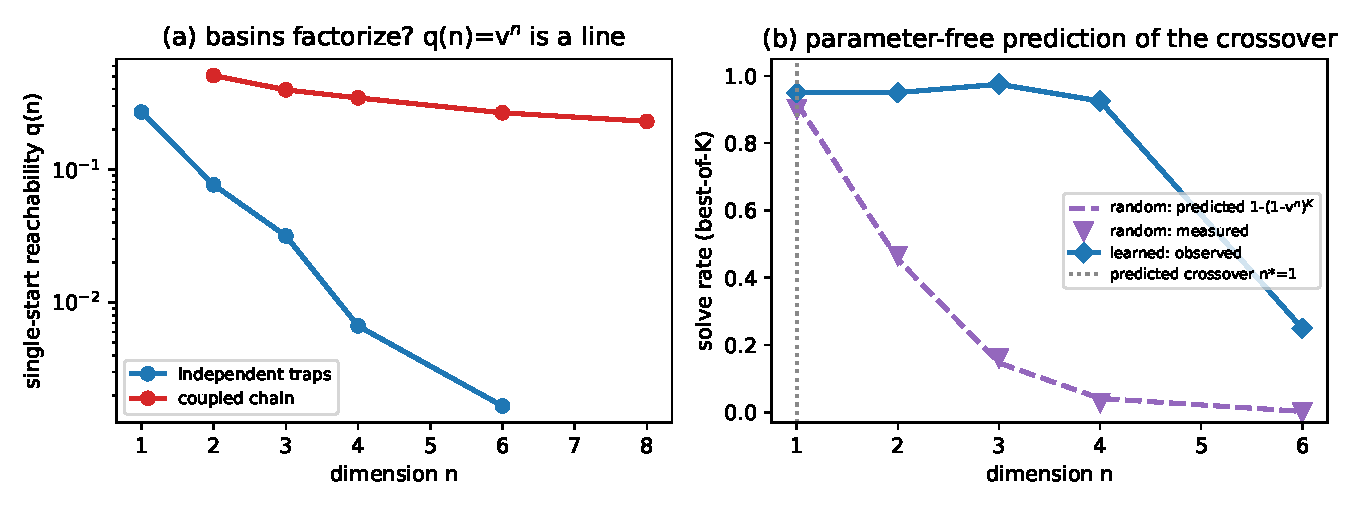
\includegraphics[width=0.62\textwidth]{../figures/fig_crossover_theory.pdf}
\caption{The factorization law, measured. Left: $\log q(n)$ against $n$. The separable family
is a line (slope $-1.03$, $R^2 = 0.98$), the coupled bilinear family is nearly flat
($-0.13$), and the geometry family, though syntactically coupled, collapses ($-0.77$,
$R^2 = 0.999$). Right: the best-of-8 random-restart curve predicted parameter-free from
$v = 0.27$ via Eq.~\eqref{eq:bestofk}, against the measured curve (MAE 0.012), with the
learned hybrid's observed solve rate overlaid; the dotted line is the crossover dimension
predicted from $v$ and the learned ceiling.}
\label{fig:law}
\end{figure*}

The separable family behaves exactly as the law requires. $\log q(n)$ is linear with slope
$-1.03$ ($R^2 = 0.98$). The parameter-free prediction uses the directly
measured $v = q(1) = 0.27$: substituting that single constant into Eq.~\eqref{eq:bestofk}
reproduces the entire best-of-8 random-restart curve with no free parameters: predicted 0.919,
0.454, 0.147, 0.042, 0.003 against the measured 0.902, 0.467, 0.162, 0.030, 0.002 at
$n = 1, 2, 3, 4, 6$, a mean absolute error of 0.012
% provenance: RESULTS.md R9 + crossover_law.md §5 (crossover_theory.json)
(Figure~\ref{fig:law}; 600 fresh instances, a larger and separately drawn sample than
Appendix Table~\ref{tab:scaling}'s $N = 40$ random arm, which runs a few
points higher at low $n$). The budget-fair
reading is the expected number of restarts $1/q(n)$: 3.7 to 600 over the separable
dimensions against 2.0--4.3 on the coupled family --- any fixed budget is exhausted on the
former, while on the latter random search never collapses and a learned proposal has
nothing to amortize. An oracle control
closes the mechanism: sampling each variable from its \emph{true} per-variable marginal
(pooled from disjoint instances) and polishing identically also ties random restart at every
$n \ge 3$ on the coupled family (0/4 significant wins). Sampling coordinates independently, it
bounds product-of-marginals proposals only, and shows population-marginal information is
exhausted here --- our denoiser behaves like a marginal sampler, not an instance-conditional
joint one. We claim no
sharp crossover at a particular $n$; the robust, predicted quantity is the geometric collapse
of the restart cost against the learned ceiling.

Separability is sufficient for geometric collapse but not necessary, so the diagnostic is the
measured slope, not the syntactic label. A real-valued geometric domain makes this concrete:
chains of unknown points ($n = 2k$ coordinates) with squared-distance constraints to fixed
anchors and between consecutive points, a non-convex quartic energy whose solutions the
checker accepts exactly. The family is syntactically coupled, yet its reachability collapses:
slope $-0.77$ ($R^2 = 0.999$), $q(n) = 0.653$, 0.147, 0.027, 0.007 at $n = 2, 4, 6, 8$
% provenance: RESULTS.md R9 (geometry) + crossover_law.md §5a
(Figure~\ref{fig:law}, left) --- each point's two-circle subproblem has a reflection
ambiguity, so a random start rarely places every point in the right basin. Collapse alone
would suggest an amortized proposal wins here. Training a denoiser on this family under the
identical protocol does not bear that out: the learned proposal ties random restart at every
chain length and collapses with it (both 0.625, 0.175, 0.025, 0.000 at $n = 2, 4, 6, 8$,
$N = 40$ per length; zero of four significant wins).
% provenance: RESULTS.md R9 (geometry) + PROVENANCE R25 (pointchain_learned.json)
The negative is the informative result, because it separates two conditions the independent
family had conflated. Reachability collapse (condition one, read off the slope) determines
whether random search fails; it does here. Separability (condition two) determines whether the
denoiser has per-variable marginals to amortize; geometry fails it, because each point's
coordinates are pinned only jointly. Both are necessary --- a learned proposal
beats classical search only where reachability collapses \emph{and} the solution is
per-variable separable --- and given those it wins when the denoiser fits the marginals:
the separable traps have both and learning wins; the coupled bilinear family fails the
first and ties; geometry has the first, fails the second, and ties. Figure~\ref{fig:regime}
places every measured family on the two axes of the law.

% provenance: paper/figures/fig_regime_map.pdf (scripts/plot_regime_map.py);
% slopes from crossover_theory.json (R9), R27 slopes law-inverted from the LM arm of
% crossover_families.json; outcomes from scaling.json (R15), crossover_families.json (R27),
% coupled.json (R7), pointchain_learned.json (R25), real_systems.json (R26)
\begin{figure}[ht]
\centering
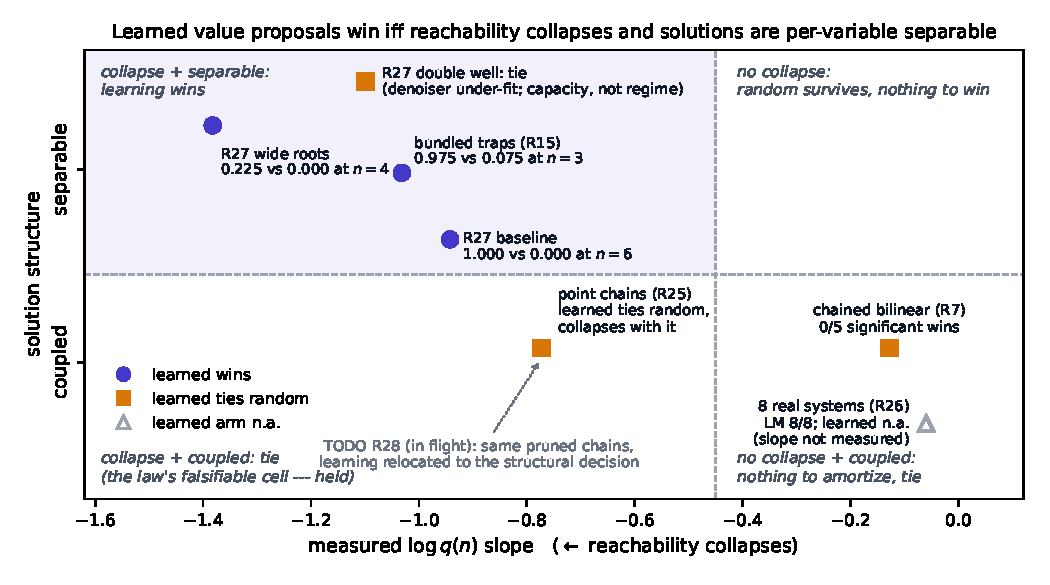
\includegraphics[width=0.88\columnwidth]{../figures/fig_regime_map.pdf}
\caption{The regime map. Each measured family sits at its measured $\log q(n)$ slope
(abscissa; the separable and coupled slopes are the fits of Table~\ref{tab:law}, the geometry slope that of Figure~\ref{fig:law}, the R27 slopes are
inverted from the best-of-8 LM arm through Eq.~\eqref{eq:bestofk}) in its solution-structure
band (ordinate, categorical), colored by the measured learned-vs-random outcome. The law
reads off the cells: learning wins only where reachability collapses \emph{and} solutions
are per-variable separable; the chained bilinear family fails collapse and ties; the
geometry point chains collapse but are coupled and tie --- the falsifiable cell, and it
held. The double-well tie inside the win cell is the capacity failure of
the dimension-scaling study, not a regime failure. The real-systems suite has no learned arm
and no measured slope (nominal abscissa); the construction-repair study took relocation to
the same pruned chains and closed it as a selection-on-noise negative (main text).}
\label{fig:regime}
\end{figure}

\subsection{Coupling removes the advantage}
\label{sec:coupled}

The law predicts where the crossover must disappear: when acceptance basins do not factorize,
$q(n)$ stays nearly flat, random restart never collapses, and a learned proposal has nothing
to amortize. The test is the coupled chained-bilinear family, $x_i + x_{i+1} = s_i$ and
$x_i \cdot x_{i+1} = p_i$, whose solution is a joint object and whose measured reachability
slope is $-0.13$ (Appendix Table~\ref{tab:law}), so what follows is a prediction checked, not
an unexplained negative. Table~\ref{tab:coupled} reports best-of-8 with 60 test instances per
$n$.

% provenance: RESULTS.md R7
\begin{table}[t]
\centering
\caption{Coupled chained-bilinear systems (best-of-8, 60 test per $n$). The learned proposal
records zero significant wins over random restart in five comparisons.}
\label{tab:coupled}
\footnotesize
\setlength{\tabcolsep}{4pt}
\begin{tabular}{ccccl}
\toprule
$n$ & Langevin & random restart & learned & learned $>$ random? \\
\midrule
2 & 0.167 & 0.483 & 0.233 & no (loses) \\
3 & 0.100 & 0.600 & 0.533 & no \\
4 & 0.050 & 0.517 & 0.517 & no (tie) \\
6 & 0.000 & 0.367 & 0.333 & no \\
8 & 0.000 & 0.467 & 0.483 & no \\
\bottomrule
\end{tabular}
\end{table}

The outcome is decisive: the learned proposal ties or loses at every
dimension, 0 significant wins out of 5. The high-dimensional advantage above
was an independence artifact --- per-variable-separable
solutions the model can memorize as marginals, and random restart forced to hit all $n$
basins by chance; coupling removes both conditions, and the proposal adds nothing over
random search plus refinement. This is the boundary of the claim.

\paragraph{Standard real systems.}
Every family above is procedurally generated, so we also ran the solver battery on eight
recognized test problems encoded once as factor graphs (circle and conic--line
intersections, GPS trilateration, Rosenbrock and Himmelblau stationary points,
2R and 3R inverse kinematics, cyclic-4), with a numeric residual tolerance
($\max_j |r_j(x)| < 10^{-6}$) since their roots are irrational.
% provenance: RESULTS.md R26 + real_systems.md (results/p_real/real_systems.json)
Multi-start Levenberg--Marquardt solves all eight; annealed Langevin solves one and random
restart with the gradient polish solves four. Where the gradient polish fails --- all at
single-start reachability $0.00$ --- the stronger \emph{classical} polish fixes every
case: the bottleneck is the finisher, not the proposal. No system falls in the amortization
regime; all are low-dimensional and coupled, so the learned component is not run per
system: nothing to amortize.

\subsection{Relocating the learned component: structural repair beats its controls}
\label{sec:repair}

Coupling closes the route where the network predicts values, and the real-systems suite
confirms classical search owns that game; the one decision classical solvers cannot make
is discrete and prior to any solve: \emph{which}
structure-changing augmentation turns an unsolvable graph into a solvable one. We move
learning there. A candidate-conditioned ranker applies each of $K$ proposed augmentations (in this
section $K$ is the menu size, not the restart budget of Eq.~\eqref{eq:bestofk}),
encodes the resulting polynomial graph with operator-aware node and edge features that expose
degree, linear/square/cross participation, and constants, and scores the augmented graphs
listwise; the highest-scoring repair receives one classical solve and the exact checker
remains the acceptance gate. A matched candidate-only control sees the same augmentation
recipe but no problem graph, and \texttt{random} chooses uniformly among the same $K$
candidates. The predecessor policy classified menu slots over one fixed graph encoding and fell to
chance on an unseen pattern; the change that matters is \emph{candidate conditioning}.
An ablation locates the signal: masking operator-identity features and
retraining leaves the ranker intact ($0.981$ vs.\ $0.997$ nonlinear, $0.379$
vs.\ $0.339$ linear) --- it lives in constants, magnitudes, and incidence read
\emph{jointly with the candidate}, not in operator flags.

% provenance: RESULTS.md R10 + PROVENANCE R20--R24; results/p_repair (Data Version 8)
\begin{table}[t]
\centering
\caption{Candidate-conditioned repair ranker against a candidate-only control and random
selection, on three generalization tests (Data Version 8; significance by exact paired McNemar in
the text). Nonlinear menus
carry exact CAS no-real-roots certificates for their distractors; every arm is graded by the
same reference solver that certified the data.}
\label{tab:repair}
\footnotesize
\setlength{\tabcolsep}{3.5pt}
\begin{tabular}{lccc}
\toprule
Test & ranker & cand.-only & random \\
\midrule
Balanced nonlinear ($N{=}360$)          & \textbf{0.997} & 0.333 & 0.236 \\
Vieta $\to$ unseen rel.\ ($N{=}150$)    & \textbf{0.420} & 0.120 & 0.253 \\
Linear, unseen pattern ($N{=}400$)      & \textbf{0.380} & 0.195 & 0.287 \\
\bottomrule
\end{tabular}
\end{table}

% provenance: paper/figures/fig_repair_accuracy.pdf (scripts/plot_repair.py --panel left)
\begin{figure}[t]
\centering
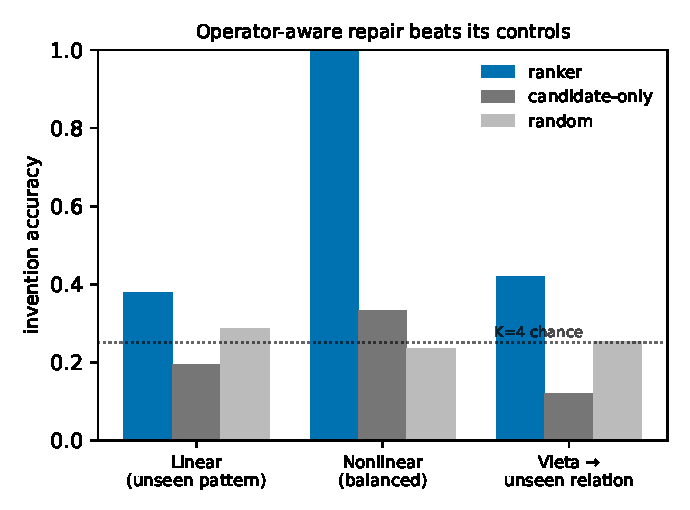
\includegraphics[width=0.8\columnwidth]{../figures/fig_repair_accuracy.pdf}
\caption{Table~\ref{tab:repair}, drawn: the ranker against its candidate-only and
random controls; the dotted line is $K{=}4$ chance. Menu-size scaling is in Appendix
Figure~\ref{fig:repair}.}
\label{fig:repair-acc}
\end{figure}

Table~\ref{tab:repair} and Figure~\ref{fig:repair-acc} report the three generalization
tests under a deliberately strict protocol (Data Version 8): one reference solver certifies the data, grades every arm,
and runs the end-to-end solves; nonlinear ``exactly one solvable option'' is an exact CAS
theorem (a distractor proven to have no real solution is unsolvable at any budget); gold and
distractor parameters share one support and one prior, so whatever surface-form signal
survives is capped at the candidate-only ceiling and anything above it must come
from reading the problem graph. On the balanced nonlinear test that ceiling is $0.333$
($N{=}360$) --- above the $0.25$ chance floor, far below the ranker,
where exact paired McNemar gives $p = 3.3\times10^{-83}$ against random (274
ranker-only correct versus 0) and $p = 1.1\times10^{-72}$ against the candidate-only
control. Transfer to an unseen nonlinear relation is partial but holds in
both directions ($0.420$ against $0.253$ for vieta-trained on quad\_link, $0.393$ against
$0.180$ for the reverse; $N{=}150$ each), not relation-level invariance. On an unseen linear
pattern the ranker reaches $0.380$ against $0.287$ ($N{=}400$); holding out each of the
other two patterns in turn gives $0.407$ and $0.450$ against
$\sim$$0.23$ random, so the effect is not specific to one holdout. A single model
tested across all three at once reads $0.339$ against $0.249$ ($N{=}1{,}200$, $p =
7.8\times10^{-7}$). The
linear signal is deliberately reported at its post-audit size: closing each discovered
shortcut lowered it ($0.565 \to 0.445 \to 0.380$ across data versions) while pushing the
candidate-only control to chance, so what remains is entirely problem-graph reading ---
modest where every operator is linear, decisive on certificate-grade nonlinear menus. Both
headline rows were retrained across three optimization seeds (11, 29, 47) with independent
per-seed evaluation draws: the nonlinear result is optimization-robust ($0.982 \pm 0.006$).
The linear edge is not seed-stable ($0.317 \pm 0.069$, one seed at $0.227$ below the random
arm's $0.248 \pm 0.002$), consistent with reading the linear rows as mechanism evidence
rather than a deployable margin.

The learned component is also cheap where value diffusion was not: one forward pass per
candidate rather than a reverse-diffusion rollout. End to end, the nonlinear ranker's single
call solves $0.933$ ---
exactly the oracle and enumeration ceiling --- where blind enumeration averages $2.62$ calls
($N{=}60$); linear $K{=}4$ solves $0.300$ against $0.227$ random with a $1.000$ ceiling
($N{=}300$). A cheap-probe control bounds the claim from the other side: a short-budget call on
every candidate solves at most $0.881$ of nonlinear menus at $4.7$ calls per instance, where
the ranker's single call solves $0.939$ ($N{=}360$) --- learning beats probing on accuracy
and cost at once, since provably rootless distractors cannot be solved at any budget while
short probes miss the gold. On linear menus the probe saturates and enumeration is
already perfect at $2.5$ calls; the $K = 4$ checkpoint transfers to larger menus without retraining but its advantage is
gone by $K = 16$, and direct $K = 16$ training sits at chance (both negatives kept in
Appendix~\ref{app:kscaling}). ``Exactly one solvable option'' is an exact certificate for all
linear menus (rank) and $99\%$ of nonlinear test menus (CAS real-root nonexistence), the
remainder carrying a disclosed budget-relative probe certificate.

% provenance: RESULTS.md R30; results/p_real_repair/real_repair{,_multiseed}.json
\paragraph{External anchor: the structural decision on systems we did not build.}
Those menus are ours. We therefore hardened four of the named real-system classes into
parameterized variants and asked whether \emph{derived} constructions --- functions of the
givens alone, law-of-cosines lifts and signed Cayley--Menger cross-product pins ---
repair the failures the classical reference cannot. Two produce a two-stream failure
population: far-side GPS trilateration ($0.848 \pm 0.020$ over three independent seed bases,
$N{=}509$ failures) and a ghost-root conic--line intersection ($0.263 \pm 0.015$, $N{=}158$);
on 3R inverse kinematics and far circles the classical solver never fails --- reported
as negatives, not averaged in as zeros. On
the two that bite, one construction chosen on a disjoint half of each failure pool repairs
\emph{every} held-out instance ($1.000 \pm 0.000$ across seeds; pooled Wilson $[0.99, 1.00]$
and $[0.98, 1.00]$) against $0.433 \pm 0.049$ and $0.114 \pm 0.011$ for a restart control
matched to the \emph{full enumeration budget} over the vocabulary (McNemar
$p < 10^{-13}$; the control, not the treatment, carries the sampling variance). The same
construction wins in all six folds, foreclosing ``the luckiest of $V$'', and saturation is
mechanical rather than fortunate --- the selected pins delete the mirror basin and the ghost
root by construction. No learned model runs: what transfers to systems we did not
design is the value of the structural decision, not the ranker.

\paragraph{Where the anchor stops: a closed negative.}
The anchor holds where the failure is a systematic attractor one construction deletes
outright; where failures are stochastic it does not, and the boundary is worth measuring.
On the pruned point chains --- the discrete-branch setting of distance geometry --- the
population definition decides the answer. Under two-stream selection ($N{=}367$
failures at the training chain lengths, three optimization seeds) the
enumeration ceiling is $0.692$ at $72.7$ restarts per instance, which plain restart scaling
matches at $+32$ ($0.725$). Majority-vote
labels made the target learnable --- the ranker separates from random ($0.246 \pm 0.016$
versus $0.185 \pm 0.019$; Holm $p{=}1.3{\times}10^{-4}$) where single-stream labels never
did --- but that is not an edge over the controls: it ties the best fixed construction
($0.259$) and loses to the matched-budget restart control ($0.270$). Real signal, and it is
the population prior; the graph adds nothing. The probe looked
like an opening: one restart per candidate solves $0.698$, matching the ceiling. But it
spends the whole menu's budget and its accepts are diffuse, so it is a portfolio sweep, not
a choice of construction --- a per-instance screen held to the reference budget scores
$0.199$ $[0.161, 0.243]$, below the restart control, so ${\sim}50$ restarts of measurement
select worse than the prior. That the learned arms land on the prior is then expected, not a
training miss: distilling the probe's labels converges there too. The gap between that honest
screen and the same screen scored on the streams that
chose it ($0.762$) is the selection-on-noise trap, measured. The verdict, read against the
anchor: a construction pays when it removes a named failure mode by construction; where none
does, constructions help only as a cheap portfolio and ``which construction''
carries no signal a selector can exploit at the reference budget.

\section{Limitations}
\label{sec:limitations}

The positive has a stated scope. The external anchor uses \emph{derived} constructions and a
held-out choice among them, not the learned ranker: it establishes that the structural
decision carries value off our benchmarks, not that our model transfers there. Its
populations are hardened variants chosen to expose a failure mode, and two of the four
classes we hardened produce no failure population at all. The ranker itself is measured on
menu-based repair over synthetic factor graphs.

On the value side, the learned
proposal's advantage requires per-variable-separable solutions and a regime where random
restart collapses; on coupled systems it never significantly beats random restart at any dimension
tested. Even on favorable families it gains nothing at $n = 1$ (random restart
at ceiling), and single cells are seed-noisy (one seed reads 0.250 at $n = 6$ where three
read $0.983 \pm 0.014$; $0.658 \pm 0.484$ at $n = 4$), so the useful window is the
crossover region,
not high dimension per se. Those separable families are also block-decomposable, so a
classical solver that read off separability would scale linearly there too; our controls use
joint starts, so the crossover is demonstrated against joint-start search, not block
decomposition. Eq.~\eqref{eq:bestofk} uses the instance-averaged $q$ (a Jensen-gap
approximation, validated against a self-measured best-of-$K$ curve) and predicts the
random-restart curve, not the learned ceiling, which is measured.

Several failures are specific and reportable. CircleLine is never solved
by the learned proposal (0.000 against 0.200 for random restart), transfer succeeds on two of
four held-out families, and adding CircleLine to the training
mix collapsed an otherwise recoverable transfer (0.70 in a smoke run to 0.00): a bad training family
actively hurts. The predecessor
structure policy never separated from random
selection; its numbers remain withdrawn (evaluation seeds overlapped checkpoint-selection
validation seeds), as do the earlier v6/v7 ranker numbers (a pin-prior leak and
probe-artifact certificates, found and fixed). The linear
edge is not stable across optimization seeds ($0.317 \pm 0.069$, one seed below the random
arm), so only the nonlinear headline ($0.982 \pm 0.006$) is optimization-robust. Finally,
scope against real problem text is quantified, not implied: on a 48-problem sample of
MATH-500 \citep{hendrycks2021math} the template formalizer covers 0 of 48 (roughly
20\% constraint-shaped, 31\% CAS computation, 48\% reasoning or proof out of
scope) --- the binding constraint is autoformalization, not the solver.
% provenance: RESULTS.md R6 (MATH prose); withdrawal provenance: RESULTS.md R8/R10

\section{Conclusion}
\label{sec:conclusion}

The decision classical solvers make only by enumeration is not which values to try but which
structure to add, and that is where learning earns its place: the repair ranker matches the
enumeration ceiling at a fraction of the calls where ``exactly one solvable option'' is a
theorem, and on hardened variants of named real systems a derived construction repairs
failures the full restart budget does not reach. On the value decision the same protocol
returns a characterization instead --- the learned proposal pays only where search is
independent across variables and dimension defeats random restart, and the advantage
disappears under coupling; what survives is the substrate and that division of labor.
The generalizable lesson is about evaluation: populations defined by stochastic failure are
artifacts of the draw unless the protocol makes them stable --- that discipline costs one
extra solve per instance, and results without it read as upper bounds.

% aaai2026.sty already sets \bibliographystyle{aaai2026}; a second one breaks bibtex
\bibliography{refs}

% ---- Technical appendix (supplementary material under AAAI rules) ----
% One-column for the wide per-family tables; the appendix ships as supplementary, not
% against the 7 content pages.
\clearpage
\onecolumn
\appendix
% aaai2026.sty sets secnumdepth to 0, which leaves \ref{app:*} empty. The main body keeps
% the kit's unnumbered headings (main-text sections are referenced by name); the appendix
% is supplementary, so restore lettering here to make "Appendix A" pointers resolve.
\setcounter{secnumdepth}{1}
% marc_aaai_appendix.tex — technical appendix for marc_aaai.tex (input after \bibliography).
% Under AAAI rules this is supplementary material; it does not count against the 7 content
% pages. Every table and number here is moved verbatim from marc.tex (port + cut, no rewrite).

\section{Per-Family Hybrid Battery and Cross-Family Transfer}
\label{app:hybrid}

The five implementation faults fixed before any comparison (the entrapment experiment): the denoiser never
received $x_t$; constants were absent from the graph tensors; $t$ did not condition variable
nodes; guidance magnitudes exploded; and a shape-handling fault in the one-variable case.
After the fixes, the solve rate on convex linear systems went from 0 to 1.000 in-distribution
and held out. A sixth, architectural fix is referenced from the Method section: per-round
LayerNorm washes out the magnitude of constraint constants, so a variable whose value is
pinned by its own constraint cannot be read off the deep features; a direct linear skip from
a variable's incident-factor constants to its output restores the path and cut the mean
absolute root error from 5.4 to 0.9.

Table~\ref{tab:hybrid} is the full mechanism ablation behind the hybrid-recipe study: four non-convex
families where deterministic descent is fully trapped (best-of-8, 60 held-out instances per
family; 95\% Wilson CIs shown on the random-init arm). The random-init control uses identical polish and budget with no
learning.

% provenance: RESULTS.md R3
\begin{table}[ht]
\centering
\caption{Mechanism ablation on trapped non-convex families (best-of-8, 60 held-out per
family; 95\% Wilson CIs on the random-init arm; columns are cold-start refinement, refinement with Langevin noise, random-init plus polish, multi-start Levenberg--Marquardt, and the learned hybrid). Values are those of the committed
\texttt{results/p\_hard/hard\_eval.json}. The multi-start Levenberg--Marquardt column is
reported for completeness: the strong classical solver saturates all four families, which is
why the learned-versus-random comparison, not the learned-versus-Langevin one, is the
informative contrast.}
\label{tab:hybrid}
\footnotesize
\setlength{\tabcolsep}{4pt}
\begin{tabular}{lccccccl}
\toprule
Family & cold & +Langevin & random-init & LM & learned & learned $>$ random? \\
\midrule
BilinearSystem  & 0.000 & 0.300 & 0.550 [0.42, 0.67] & 1.000 & 0.550 & tie ($p{=}0.50$) \\
BilinearProduct & 0.000 & 0.100 & 0.683 [0.56, 0.79] & 1.000 & 0.683 & tie ($p{=}0.50$) \\
QuadraticSystem & 0.000 & 0.300 & 0.683 [0.56, 0.79] & 1.000 & 0.683 & tie ($p{=}0.50$) \\
CircleLine      & 0.000 & 0.033 & 0.200 [0.12, 0.32] & 1.000 & 0.000 & no (random wins) \\
\bottomrule
\end{tabular}
\end{table}

\label{app:transfer}
Cross-family transfer is partial. We train on three non-convex families and test the hybrid
on the held-out fourth (best-of-8, 60 test instances per family, 200 epochs);
Table~\ref{tab:transfer} reports the outcome. On two of four held-out families the
cross-trained model reaches 0.683, significantly above the refine+Langevin baseline
($p < 10^{-4}$): the model solves a family it never trained on. On the other two it solves
nothing. The BilinearSystem failure is the informative one, because that family is solvable
in-distribution (0.550 in Table~\ref{tab:hybrid}). A smoke run trained on only the two
similar families \{Product, Quadratic\} recovered it at 0.70, whereas adding the pathological
CircleLine family to the training mix collapsed it to 0.00. Dissimilar training families can
degrade transfer. We read this as transfer across related non-convex structure, not
as a universal solver.

% provenance: RESULTS.md R4
\begin{table}[ht]
\centering
\caption{Leave-one-family-out transfer (best-of-8, 60 test per family, 200 epochs). $p$ from
a $z$-test of learned (cross) $>$ refine+Langevin.}
\label{tab:transfer}
\small
\begin{tabular}{lllll}
\toprule
Held-out family & Trained on & refine+Langevin & learned (cross) & $p$ \\
\midrule
BilinearProduct & Sys, Quad, Circle  & 0.100 [0.05, 0.20] & 0.683 [0.56, 0.79] & $<10^{-4}$ \\
QuadraticSystem & Sys, Prod, Circle  & 0.300 [0.20, 0.43] & 0.683 [0.56, 0.79] & $<10^{-4}$ \\
BilinearSystem  & Prod, Quad, Circle & 0.300 [0.20, 0.43] & 0.000 & fails \\
CircleLine      & Sys, Prod, Quad    & 0.033 [0.01, 0.11] & 0.000 & fails \\
\bottomrule
\end{tabular}
\end{table}

\section{Dimension Scaling: Full Battery}
\label{app:scaling}

Table~\ref{tab:scaling} is the full five-arm battery behind the dimension-scaling study; the main text and
Figure 1 of the main paper carry the two arms that decide the claim (random restart and learned).

% provenance: RESULTS.md R15 (methodology unified-v2, results/p_scaling/scaling.json)
\begin{table}[ht]
\centering
\caption{Dimension scaling on bundled traps with per-instance-varying roots in $\pm[3,8]$
(best-of-8, unified-v2 protocol: one shared polish and one checker for every arm, $N{=}40$
per cell; 95\% Wilson half-widths are at most $0.15$). Bold marks the best method per
row. A three-seed rerun of the same protocol ($N{=}120$ per cell,
scaling\_3seed.json) reads $0.983 \pm 0.014$ at $n{=}6$ and $0.658 \pm 0.484$ at
$n{=}4$: single cells are seed-noisy, the crossover is not.}
\label{tab:scaling}
\begin{tabular}{cccccc}
\toprule
$n$ & deterministic & Langevin & mean-prior & random restart & learned \\
\midrule
1 & 0.000 & 0.775 & 0.000 & \textbf{1.000} & 0.950 \\
2 & 0.000 & 0.225 & 0.000 & 0.725 & \textbf{0.950} \\
3 & 0.000 & 0.000 & 0.000 & 0.075 & \textbf{0.975} \\
4 & 0.000 & 0.000 & 0.000 & 0.000 & \textbf{0.925} \\
6 & 0.000 & 0.000 & 0.000 & 0.000 & \textbf{0.250} \\
\bottomrule
\end{tabular}
\end{table}

\section{The Factorization Dichotomy: Regime Map and Table}
\label{app:law}

The regime map (Figure 2 of the main paper) places every measured family on the
two axes of the law; Table~\ref{tab:law} tabulates the dichotomy plotted in
Figure 1 of the main paper (600 fresh instances per $n$, Wilson CIs, $K = 8$). Expected restarts
$1/q(n)$ are listed over the tested dimensions in increasing order.

Slope provenance for the regime map: the separable and coupled abscissae are the fits of
Table~\ref{tab:law}, the geometry abscissa is the fit of Figure 1 of the main paper, and the
three crossover-replication families are placed at slopes inverted from their best-of-8
Levenberg--Marquardt arm through the best-of-$K$ identity of the main paper. The real-systems suite is plotted
at a nominal abscissa: it has no learned arm and no separately measured $q(n)$.


% provenance: RESULTS.md R9 + paper/notes/crossover_law.md §5
\begin{table}[ht]
\centering
\caption{The factorization dichotomy, measured.}
\label{tab:law}
\small
\begin{tabular}{lll}
\toprule
Quantity & Independent (separable) & Coupled \\
\midrule
$\log q(n)$ slope & $-1.03$ & $-0.13$ \\
fit $R^2$ & 0.98 & 0.96 \\
measured $v = q(1)$ & 0.27 & --- \\
$E[\text{starts}] = 1/q(n)$ & $3.7 \to 13 \to 32 \to 150 \to 600$ & $2.0 \to 2.5 \to 2.9 \to 3.8 \to 4.3$ \\
$P_{\text{random}}$ MAE, parameter-free & 0.012 & law N/A (not separable) \\
\bottomrule
\end{tabular}
\end{table}

\section{External Anchor: Per-Class Construction Repair}
\label{app:anchor}

Table~\ref{tab:anchor} is the per-class breakdown behind the external-anchor paragraph.
Both restart controls rerun the same classical reference solver on the unrepaired system:
\texttt{restart} at the reference solver's own budget, \texttt{restart}$\times|V|$ at the
full enumeration budget over the construction vocabulary. The two classes that never fail
are reported as negatives rather than averaged in as zeros; the own-budget column shows how
far short a plain retry falls even before the budget is matched.

% provenance: RESULTS.md R30; results/p_real_repair/real_repair_multiseed.json (aggregate)
\begin{table}[ht]
\centering
\caption{Derived-construction repair on hardened variants of named real systems: three
independent seed bases, $N{=}200$ instances per class per seed, mean $\pm$ population SD.
``Failures'' is the two-stream failure rate of the classical reference and $N$ the pooled
failure population it defines; the construction is chosen on a disjoint half of that pool
and graded on the held-out half.}
\label{tab:anchor}
\small
\begin{tabular}{lrrccc}
\toprule
Class & Failures & $N$ & construction (held out) & restart & restart$\times|V|$ \\
\midrule
Trilateration, far side & $0.848 \pm 0.020$ & 509 & $\mathbf{1.000 \pm 0.000}$
  & $0.079 \pm 0.017$ & $0.433 \pm 0.049$ \\
Conic--line, ghost root & $0.263 \pm 0.015$ & 158 & $\mathbf{1.000 \pm 0.000}$
  & $0.026 \pm 0.010$ & $0.114 \pm 0.011$ \\
3R inverse kinematics & $0.000$ & 0 & --- & --- & --- \\
Circles, far apart & $0.000$ & 0 & --- & --- & --- \\
\bottomrule
\end{tabular}
\end{table}

\section{Repair: Menu-Size Scaling and Cost Accounting}
\label{app:kscaling}

The $K{=}4$ checkpoint transfers to larger linear menus without retraining, but the accuracy
advantage shrinks with $K$ and is gone by $K{=}16$ ($0.300/0.187/0.113$ against random
$0.227/0.120/0.107$ at $K{=}4/8/16$, $N{=}300/150/150$); what survives at large $K$ is only
the cost gap, as the enumeration it displaces grows to $9.05$ solver calls per instance
(Figure~\ref{fig:repair}). Directly training at $K{=}16$ performs at chance, so the
transferred checkpoint is selected and both negatives are kept in the record.

% provenance: paper/tex/figures/fig_repair.pdf (scripts/plot_repair.py), RESULTS.md R10
\begin{figure}[t]
\centering

\includegraphics[width=0.85\textwidth]{figures/fig_repair.pdf}
\caption{Left: Table 3 of the main paper drawn, the ranker against its
candidate-only and random controls, with $K{=}4$ chance dotted. Right: menu-size scaling.
The $K{=}4$ checkpoint evaluated zero-shot at larger menus retains an accuracy edge at
$K{=}8$ that closes by $K{=}16$, while the blind enumeration it displaces grows from $2.5$
to $9.1$ solver calls per instance.}
\label{fig:repair}
\end{figure}

\section{MATH-500 Scope Measurement}
\label{app:math}

The main text states that the template formalizer covers none of a 48-problem MATH-500
sample \citep{hendrycks2021math}. The breakdown: roughly $20\%$ of the sample is
constraint-shaped and in principle in scope, $31\%$ is CAS computation rather than
constraint solving, and $48\%$ is reasoning or proof that the factor-graph encoding does
not express. Coverage is $0/48$ because the constraint-shaped fraction still requires
autoformalization from problem text, which the template formalizer does not perform. The
binding constraint on applying this substrate to natural problem statements is therefore
autoformalization, not the solver.
% provenance: RESULTS.md R6 / PROVENANCE R14 (scripts/run_math_coverage.py)


\end{document}
